% Editable native annotations around unchanged verified IDE photographs.
\par
\begin{figure}[htbp]
  \centering
  \newsavebox{\MARSbaseSixtyFourpairregistersBox}
  \sbox{\MARSbaseSixtyFourpairregistersBox}{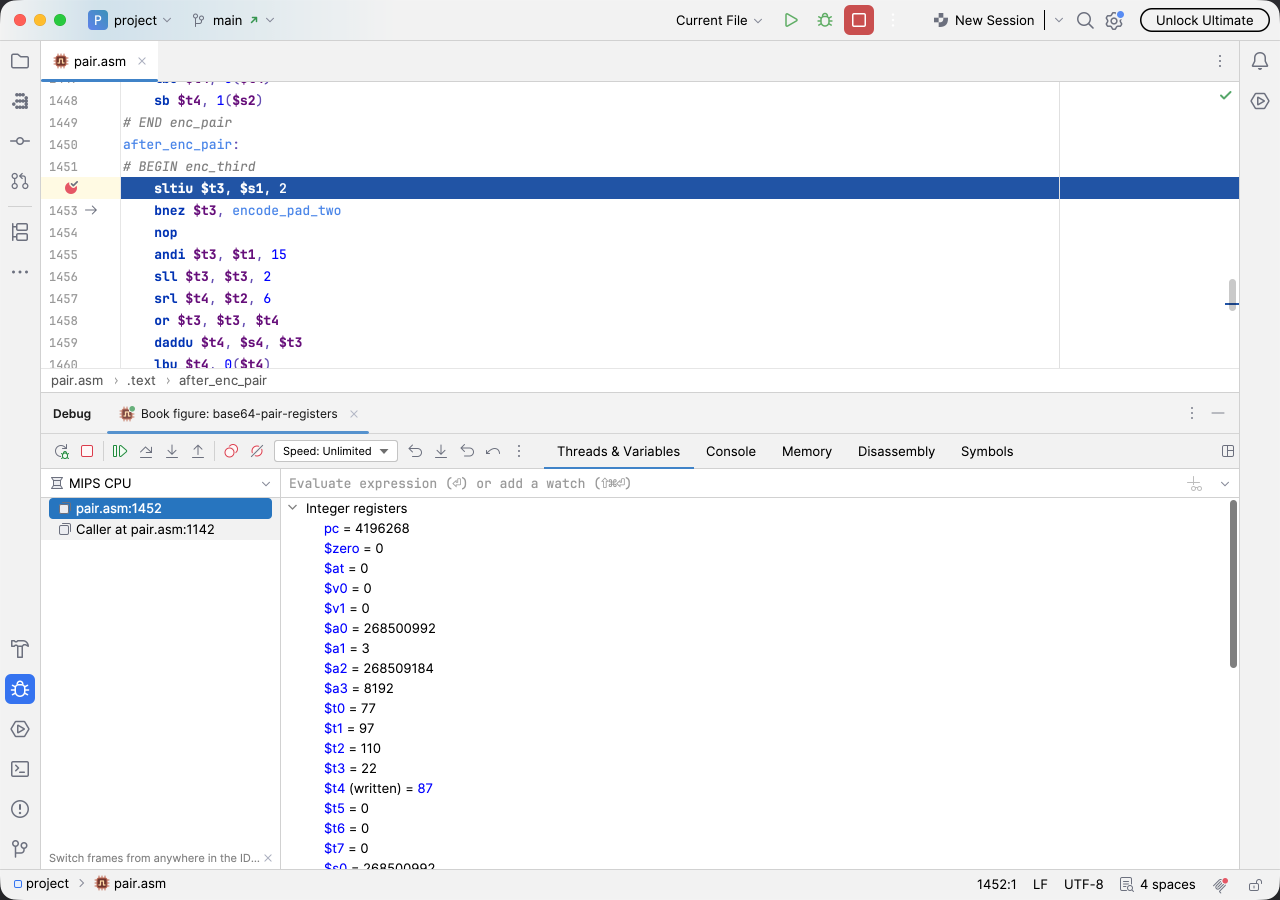
\includegraphics[artifact]{packages/028-base64/captures/f01/registers.png}}
  \newsavebox{\MARSbaseSixtyFourpairsourceBox}
  \sbox{\MARSbaseSixtyFourpairsourceBox}{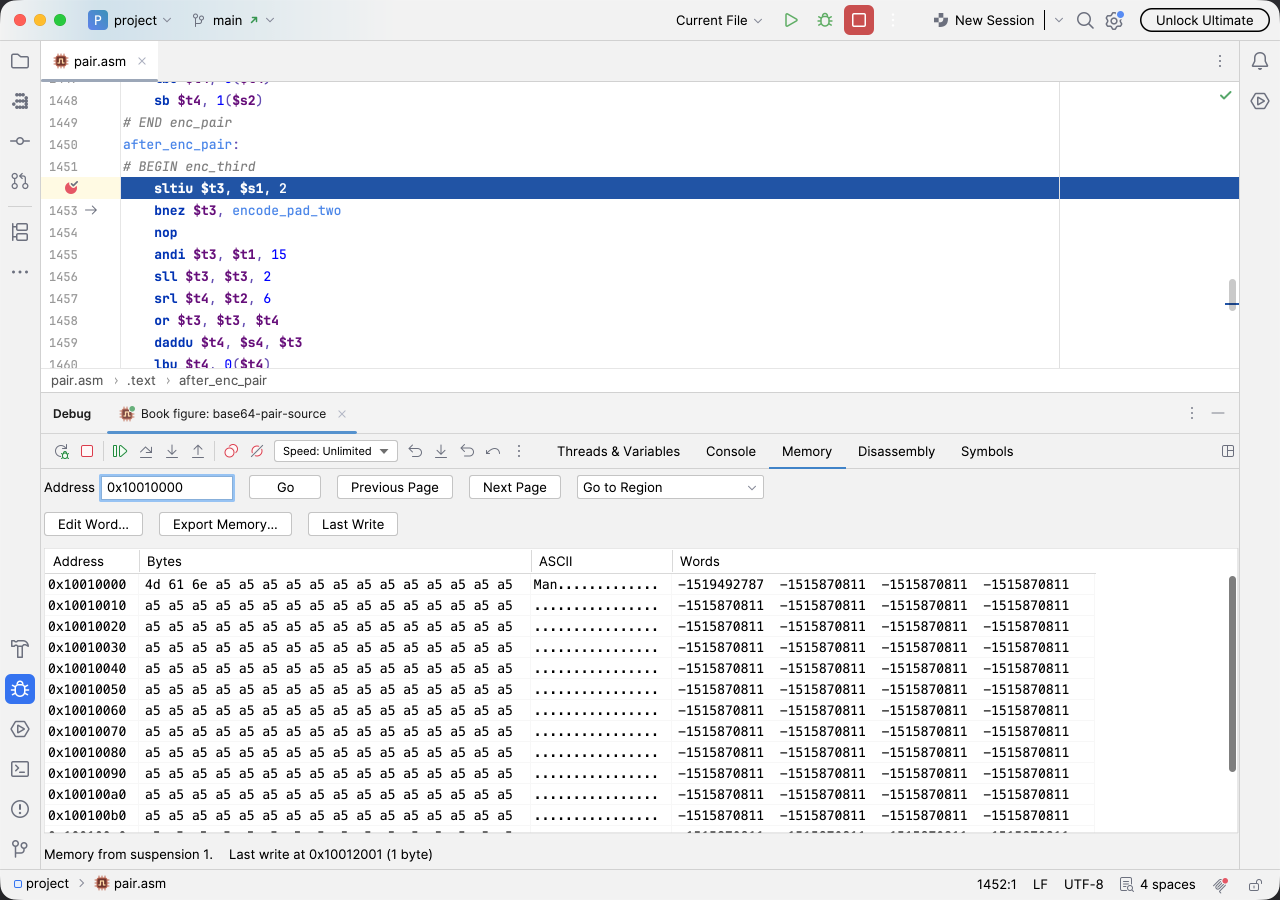
\includegraphics[artifact]{packages/028-base64/captures/f01/source.png}}
  \newsavebox{\MARSbaseSixtyFourpairoutputBox}
  \sbox{\MARSbaseSixtyFourpairoutputBox}{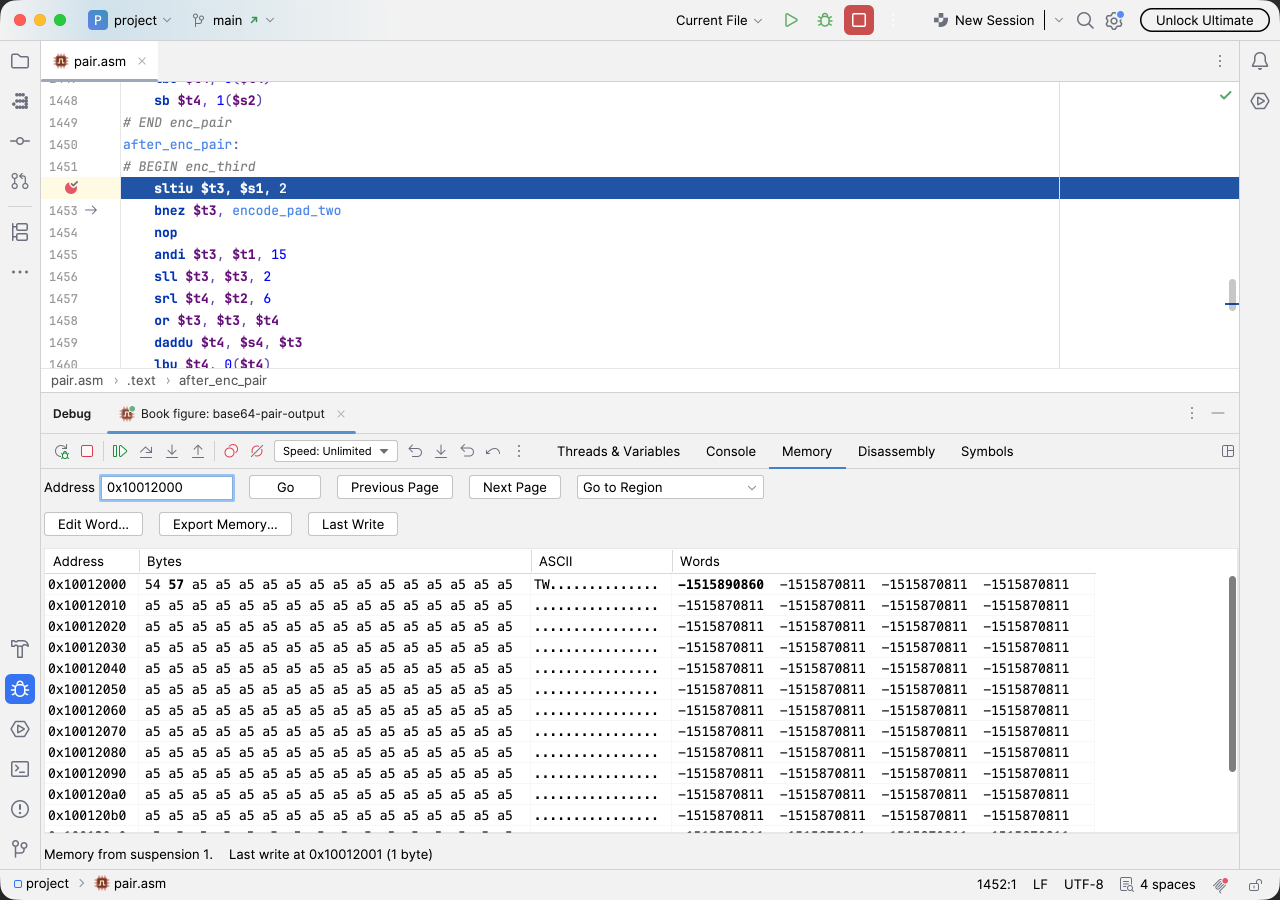
\includegraphics[artifact]{packages/028-base64/captures/f01/output.png}}
  \newsavebox{\MARSbaseSixtyFourpairalphabetBox}
  \sbox{\MARSbaseSixtyFourpairalphabetBox}{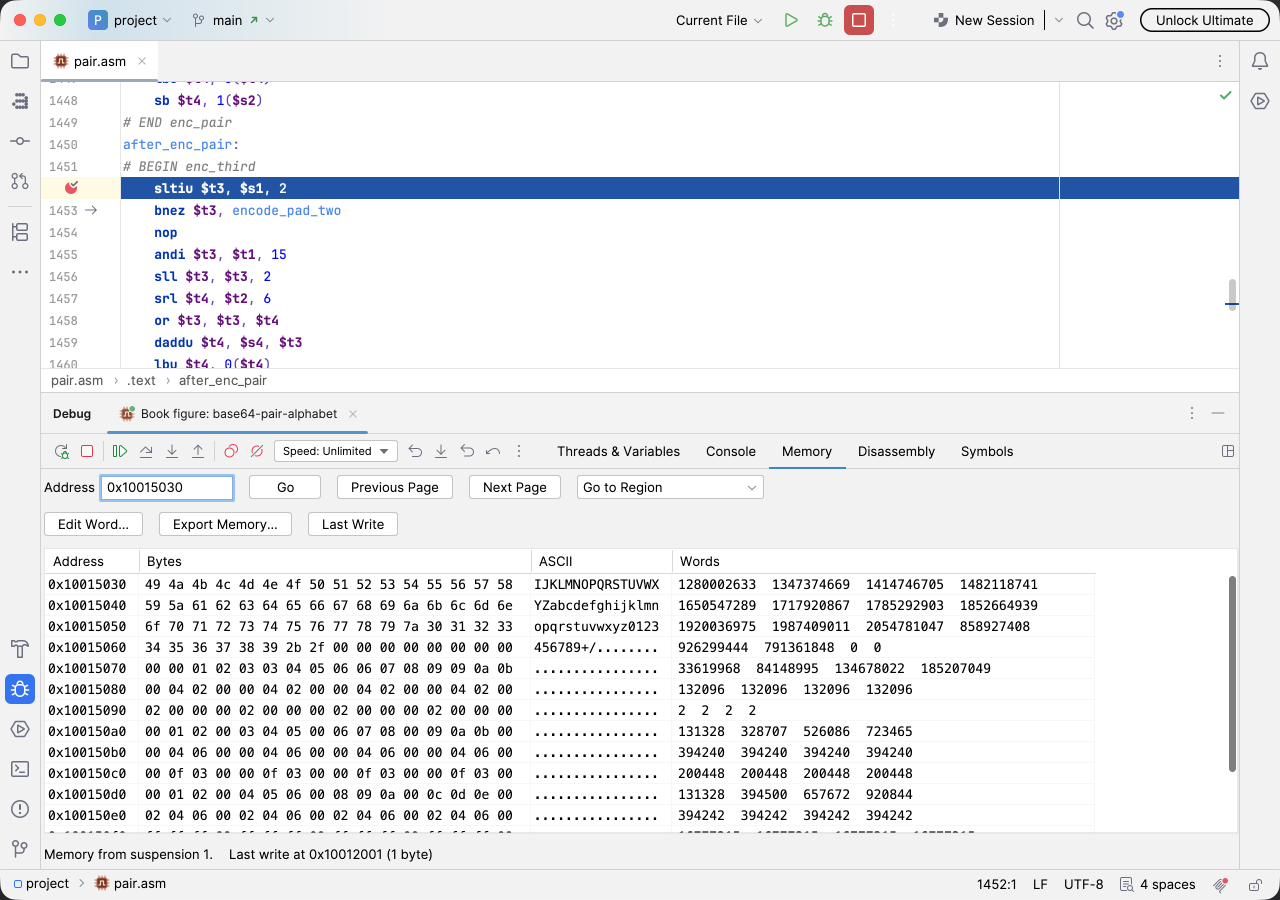
\includegraphics[artifact]{packages/028-base64/captures/f01/alphabet.png}}
  \edef\MARSbaseSixtyFourpairsourceLeft{\the\dimexpr0.036718750\wd\MARSbaseSixtyFourpairregistersBox\relax}
  \edef\MARSbaseSixtyFourpairsourceBottom{\the\dimexpr0.774444444\ht\MARSbaseSixtyFourpairregistersBox\relax}
  \edef\MARSbaseSixtyFourpairsourceRight{\the\dimexpr0.713281250\wd\MARSbaseSixtyFourpairregistersBox\relax}
  \edef\MARSbaseSixtyFourpairsourceTop{\the\dimexpr0.170000000\ht\MARSbaseSixtyFourpairregistersBox\relax}
  \edef\MARSbaseSixtyFourpairreturnsLeft{\the\dimexpr0.246093750\wd\MARSbaseSixtyFourpairregistersBox\relax}
  \edef\MARSbaseSixtyFourpairreturnsBottom{\the\dimexpr0.112222222\ht\MARSbaseSixtyFourpairregistersBox\relax}
  \edef\MARSbaseSixtyFourpairreturnsRight{\the\dimexpr0.553906250\wd\MARSbaseSixtyFourpairregistersBox\relax}
  \edef\MARSbaseSixtyFourpairreturnsTop{\the\dimexpr0.840000000\ht\MARSbaseSixtyFourpairregistersBox\relax}
  \edef\MARSbaseSixtyFourpairinputLeft{\the\dimexpr0.034375000\wd\MARSbaseSixtyFourpairsourceBox\relax}
  \edef\MARSbaseSixtyFourpairinputBottom{\the\dimexpr0.334444444\ht\MARSbaseSixtyFourpairsourceBox\relax}
  \edef\MARSbaseSixtyFourpairinputRight{\the\dimexpr0.584375000\wd\MARSbaseSixtyFourpairsourceBox\relax}
  \edef\MARSbaseSixtyFourpairinputTop{\the\dimexpr0.608888889\ht\MARSbaseSixtyFourpairsourceBox\relax}
  \edef\MARSbaseSixtyFourpairalphabetLeft{\the\dimexpr0.034375000\wd\MARSbaseSixtyFourpairalphabetBox\relax}
  \edef\MARSbaseSixtyFourpairalphabetBottom{\the\dimexpr0.334444444\ht\MARSbaseSixtyFourpairalphabetBox\relax}
  \edef\MARSbaseSixtyFourpairalphabetRight{\the\dimexpr0.584375000\wd\MARSbaseSixtyFourpairalphabetBox\relax}
  \edef\MARSbaseSixtyFourpairalphabetTop{\the\dimexpr0.608888889\ht\MARSbaseSixtyFourpairalphabetBox\relax}
  \edef\MARSbaseSixtyFourpairoutputLeft{\the\dimexpr0.034375000\wd\MARSbaseSixtyFourpairoutputBox\relax}
  \edef\MARSbaseSixtyFourpairoutputBottom{\the\dimexpr0.334444444\ht\MARSbaseSixtyFourpairoutputBox\relax}
  \edef\MARSbaseSixtyFourpairoutputRight{\the\dimexpr0.584375000\wd\MARSbaseSixtyFourpairoutputBox\relax}
  \edef\MARSbaseSixtyFourpairoutputTop{\the\dimexpr0.608888889\ht\MARSbaseSixtyFourpairoutputBox\relax}
  \begin{tikzpicture}[alt={Five annotated details after_enc_pair show source bytes 4d616e for Man, second sextet 22, ASCII value 87 for W, alphabet entries including T and W, and output bytes 54 57 followed by untouched a5 bytes. Two characters of the eventual TWFu output have been stored.}]
    \node[anchor=north west,inner sep=0,font=\small\bfseries] (source-title) at (6mm,0) {Next scalar encoder instruction};
    \node[anchor=north west,inner sep=0] (source) at ([yshift=-1mm]source-title.south west) {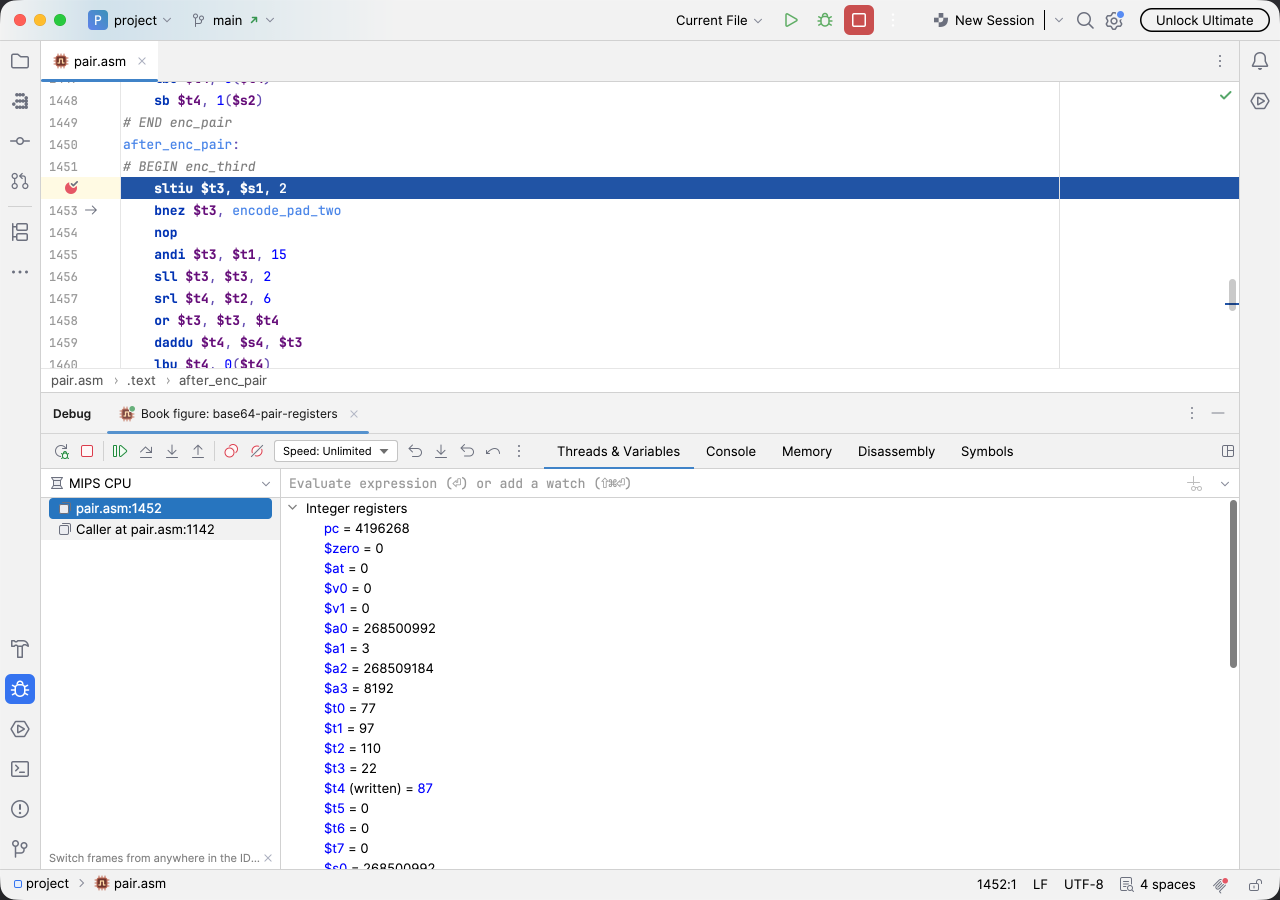
\includegraphics[width=0.54\linewidth,artifact,trim={\MARSbaseSixtyFourpairsourceLeft{} \MARSbaseSixtyFourpairsourceBottom{} \MARSbaseSixtyFourpairsourceRight{} \MARSbaseSixtyFourpairsourceTop{}},clip]{packages/028-base64/captures/f01/registers.png}};
    \begin{scope}[shift={(source.south west)},x={($(source.south east)-(source.south west)$)},y={($(source.north west)-(source.south west)$)}]
      \draw[black,line width=0.7pt] (0.237500000,0.080000000) rectangle (0.746875000,0.520000000);
      \node[draw=black,fill=white,circle,inner sep=1.5pt,font=\footnotesize] at ($(0.237500000,0.520000000)+(-3mm,0)$) {1};
    \end{scope}
    \node[anchor=north west,inner sep=0,font=\small\bfseries] (returns-title) at ([yshift=-1mm]source.south west) {Second sextet and looked-up character};
    \node[anchor=north west,inner sep=0] (returns) at ([yshift=-1mm]returns-title.south west) {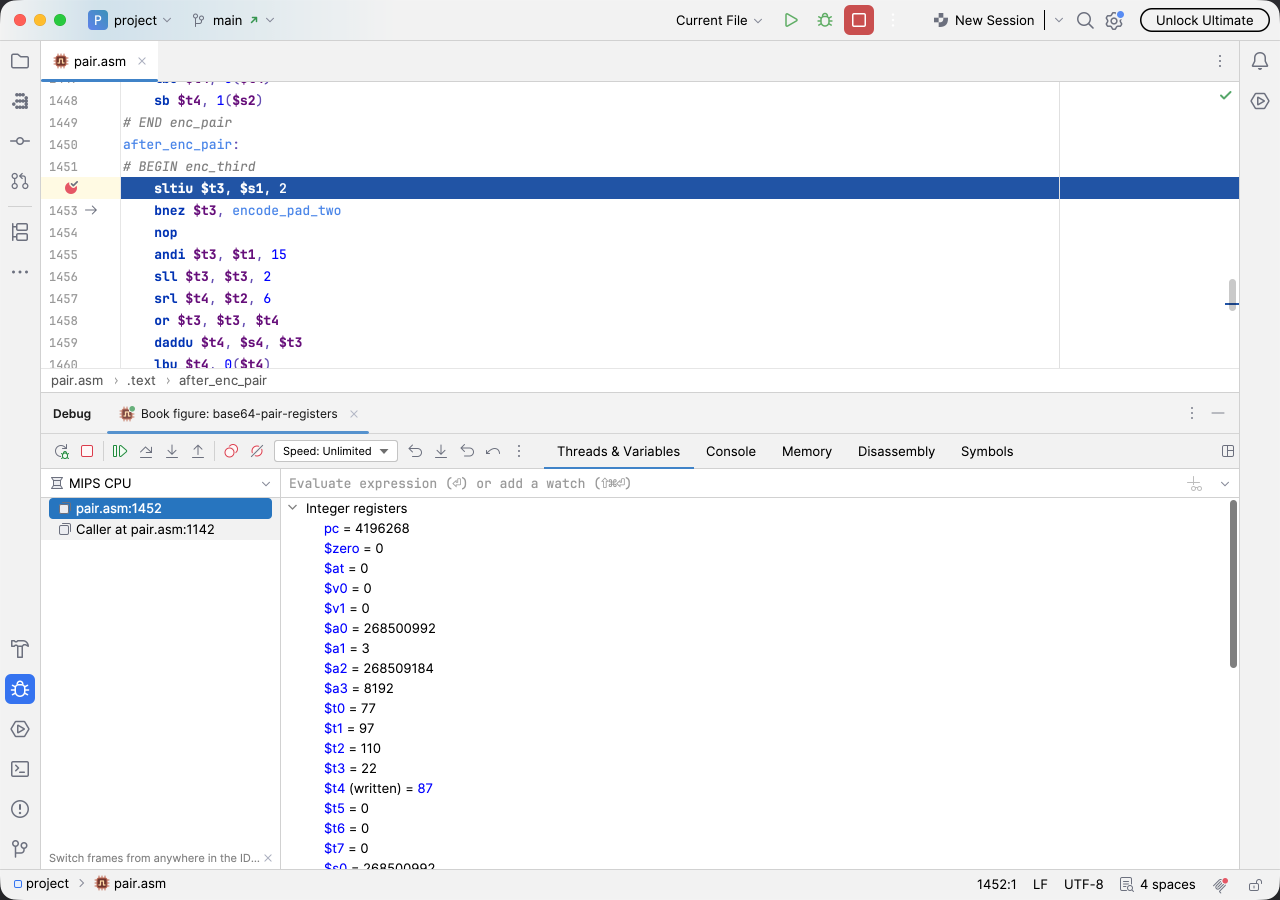
\includegraphics[width=0.44\linewidth,artifact,trim={\MARSbaseSixtyFourpairreturnsLeft{} \MARSbaseSixtyFourpairreturnsBottom{} \MARSbaseSixtyFourpairreturnsRight{} \MARSbaseSixtyFourpairreturnsTop{}},clip]{packages/028-base64/captures/f01/registers.png}};
    \begin{scope}[shift={(returns.south west)},x={($(returns.south east)-(returns.south west)$)},y={($(returns.north west)-(returns.south west)$)}]
      \draw[black,line width=0.7pt] (0.023437500,0.023255814) rectangle (0.464843750,0.953488372);
      \node[draw=black,fill=white,circle,inner sep=1.5pt,font=\footnotesize] at ($(0.023437500,0.953488372)+(-3mm,0)$) {2};
    \end{scope}
    \node[anchor=north west,inner sep=0,font=\small\bfseries] (input-title) at ([yshift=-1mm]returns.south west) {Three source bytes and backing suffix};
    \node[anchor=north west,inner sep=0] (input) at ([yshift=-1mm]input-title.south west) {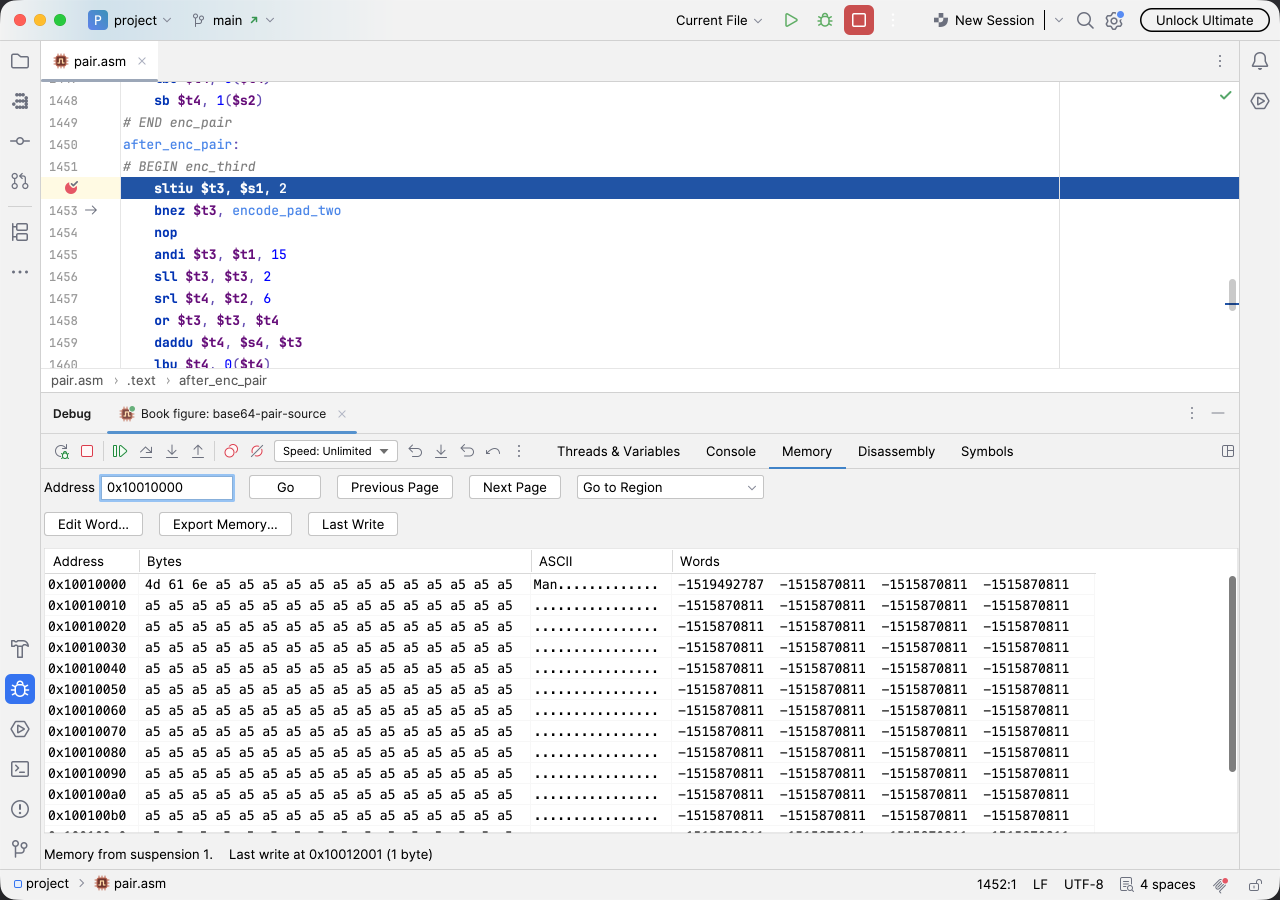
\includegraphics[width=0.84\linewidth,artifact,trim={\MARSbaseSixtyFourpairinputLeft{} \MARSbaseSixtyFourpairinputBottom{} \MARSbaseSixtyFourpairinputRight{} \MARSbaseSixtyFourpairinputTop{}},clip]{packages/028-base64/captures/f01/source.png}};
    \begin{scope}[shift={(input.south west)},x={($(input.south east)-(input.south west)$)},y={($(input.north west)-(input.south west)$)}]
      \draw[black,line width=0.7pt] (0.194672131,0.078431373) rectangle (0.997950820,0.490196078);
      \node[draw=black,fill=white,circle,inner sep=1.5pt,font=\footnotesize] at ($(0,0.490196078)+(-3mm,0)$) {3};
    \end{scope}
    \node[anchor=north west,inner sep=0,font=\small\bfseries] (alphabet-title) at ([yshift=-1mm]input.south west) {Alphabet entries eight through twenty-three};
    \node[anchor=north west,inner sep=0] (alphabet) at ([yshift=-1mm]alphabet-title.south west) {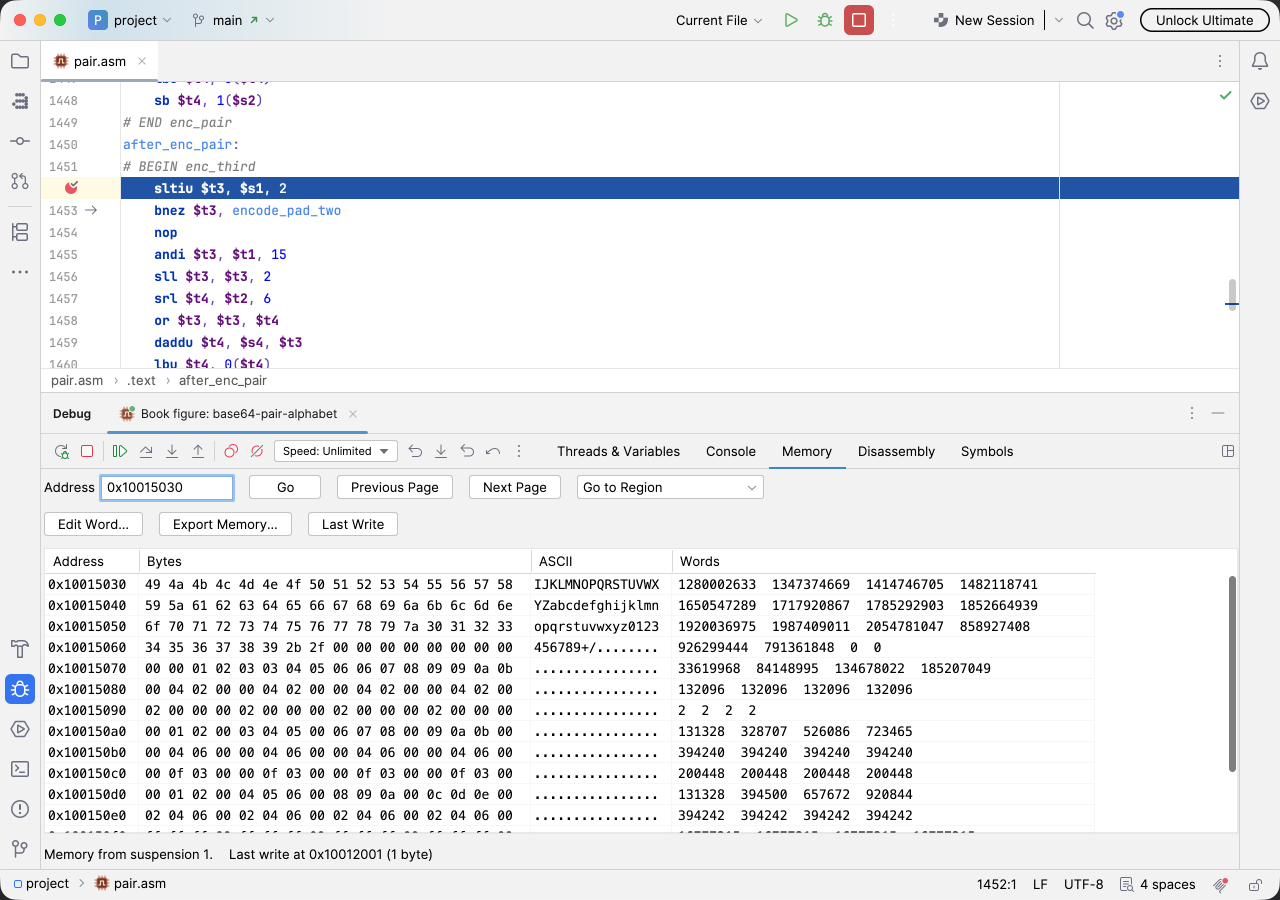
\includegraphics[width=0.84\linewidth,artifact,trim={\MARSbaseSixtyFourpairalphabetLeft{} \MARSbaseSixtyFourpairalphabetBottom{} \MARSbaseSixtyFourpairalphabetRight{} \MARSbaseSixtyFourpairalphabetTop{}},clip]{packages/028-base64/captures/f01/alphabet.png}};
    \begin{scope}[shift={(alphabet.south west)},x={($(alphabet.south east)-(alphabet.south west)$)},y={($(alphabet.north west)-(alphabet.south west)$)}]
      \draw[black,line width=0.7pt] (0.194672131,0.078431373) rectangle (0.997950820,0.490196078);
      \node[draw=black,fill=white,circle,inner sep=1.5pt,font=\footnotesize] at ($(0,0.490196078)+(-3mm,0)$) {4};
    \end{scope}
    \node[anchor=north west,inner sep=0,font=\small\bfseries] (output-title) at ([yshift=-1mm]alphabet.south west) {Published two-character prefix};
    \node[anchor=north west,inner sep=0] (output) at ([yshift=-1mm]output-title.south west) {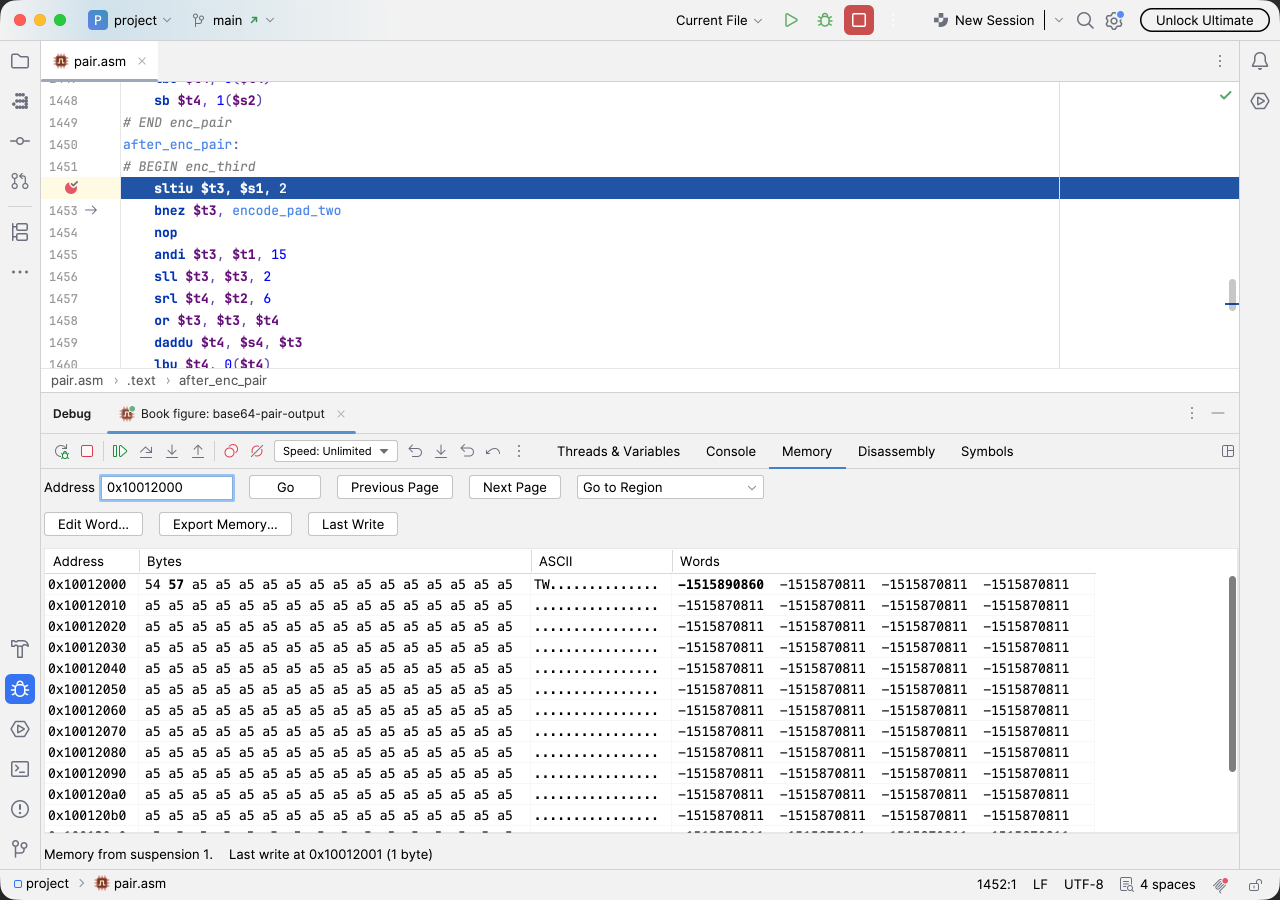
\includegraphics[width=0.84\linewidth,artifact,trim={\MARSbaseSixtyFourpairoutputLeft{} \MARSbaseSixtyFourpairoutputBottom{} \MARSbaseSixtyFourpairoutputRight{} \MARSbaseSixtyFourpairoutputTop{}},clip]{packages/028-base64/captures/f01/output.png}};
    \begin{scope}[shift={(output.south west)},x={($(output.south east)-(output.south west)$)},y={($(output.north west)-(output.south west)$)}]
      \draw[black,line width=0.7pt] (0.194672131,0.078431373) rectangle (0.997950820,0.490196078);
      \node[draw=black,fill=white,circle,inner sep=1.5pt,font=\footnotesize] at ($(0,0.490196078)+(-3mm,0)$) {5};
    \end{scope}
  \end{tikzpicture}
  \par\smallskip
  \begin{minipage}{\linewidth}
    \small
    \begin{enumerate}
      \setlength{\itemsep}{0pt}
            \setlength{\parsep}{0pt}
      \item At \texttt{after\_enc\_pair}, the first two characters are stored. The next region constructs the third sextet; this is an intermediate output prefix.
      \item \texttt{t3 = 22} is a numerical sextet. Looking up alphabet entry 22 gives ASCII \texttt{W}, whose decimal code 87 is in \texttt{t4}. A sextet value and its encoded character are different representations.
      \item The source begins \texttt{4d 61 6e}, the bytes of \texttt{Man}. The following \texttt{a5} bytes are outside its three-byte logical input.
      \item This alphabet row begins with entry 8, \texttt{I}. Entry 19 is \texttt{T}; entry 22 is \texttt{W}. Memory holds character codes, while the sextets supply indices into this table.
      \item The output starts \texttt{54 57}, ASCII \texttt{TW}. All later destination bytes remain \texttt{a5}. Continuing completes \texttt{TWFu} and returns a written count of four; no string terminator is part of that output.
    \end{enumerate}
  \end{minipage}
  \caption{Two scalar alphabet lookups publish the prefix before the group is complete.}
  \label{capture:028-base64-f01}
  \label{base64-f01}
\end{figure}
\par
